\section{Results}\label{sec:results}

\begin{figure}[!htbp]
\centering
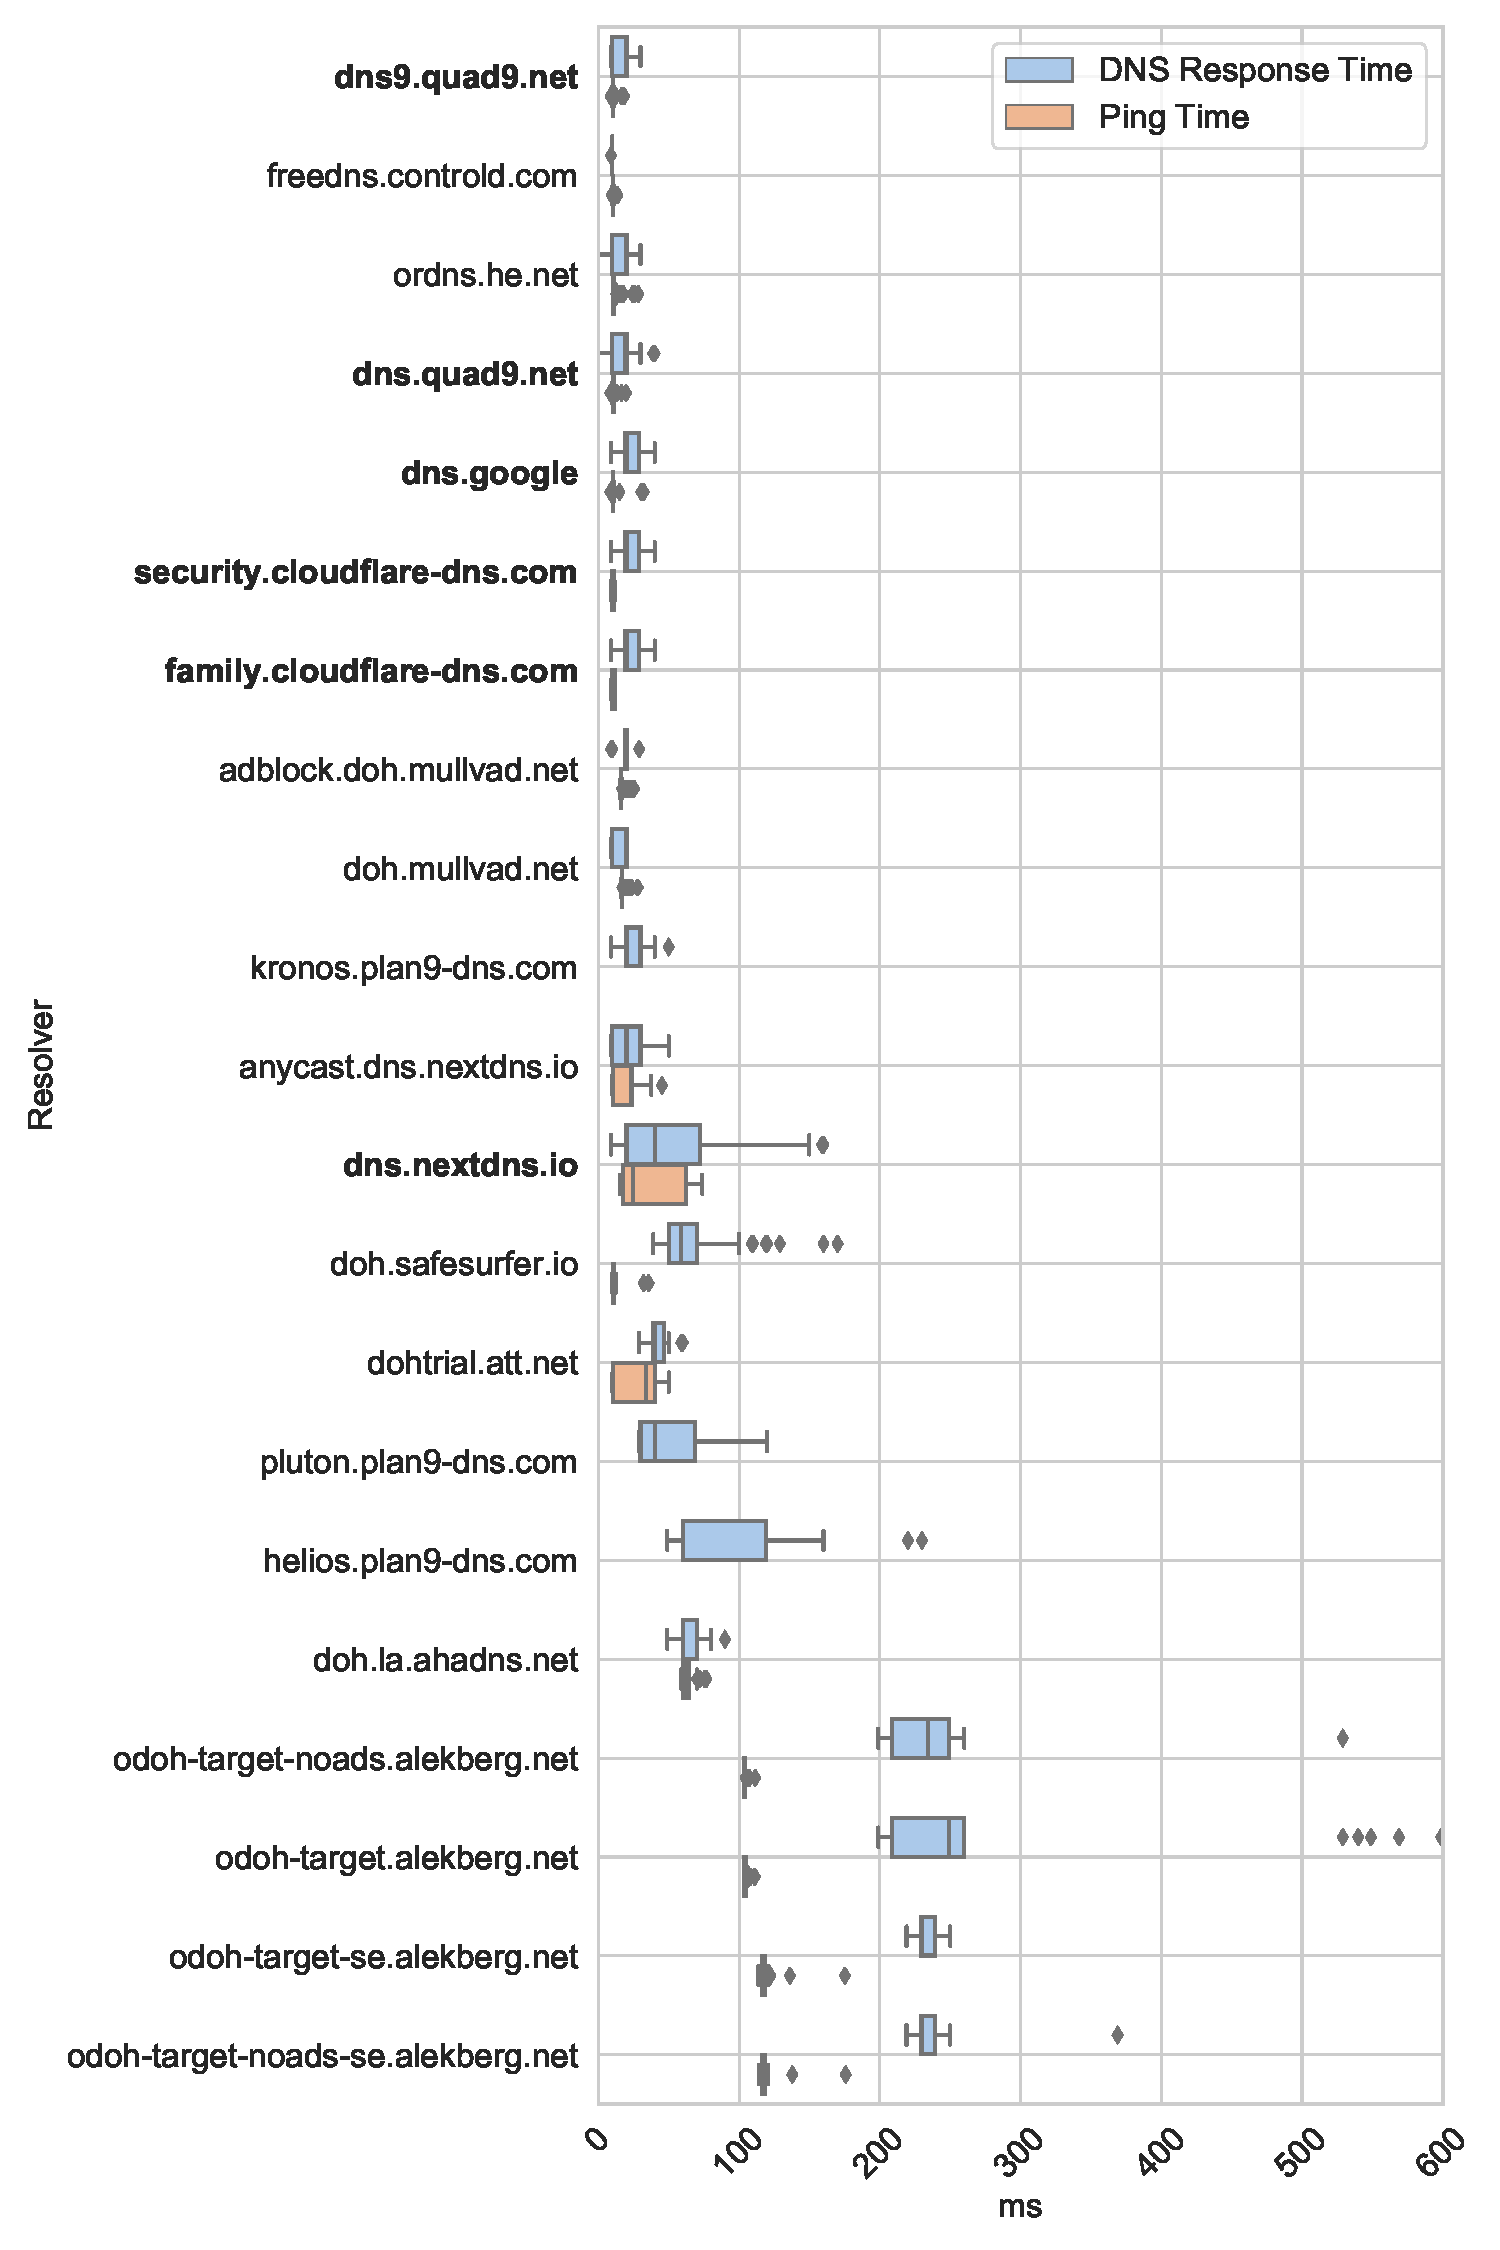
\includegraphics[width=0.6\columnwidth]{figures/ohio_NA.pdf}
\caption{DNS response time and ICMP ping time distributions for
    encrypted DNS resolvers located in North America, measured from EC2 in Ohio. Mainstream resolvers are bolded.}
    \label{fig:dns-us-ohio}
\end{figure}

Figure~\ref{fig:dns-us-ohio} shows the distributions of DNS response times and
ICMP ping times across encrypted DNS resolvers located in North America, as
measured from an EC2 instance in Ohio. The plots show distributions for both DNS response times and ICMP round-trip latency.

As expected, most mainstream resolvers outperformed non-mainstream resolvers from most vantage points. Non-mainstream resolvers also exhibited higher variability of median query response times. In some cases, however, a local non-mainstream resolver can exhibit equivalent performance as compared mainstream resolvers (e.g., ordns.he.net, freedns.controld.com, dns.brahma.world, and dns.alidns.com). These results suggest both good news and room for improvement in the future: On the one hand, viable alternatives to mainstream encrypted DNS resolvers do exist. On the other hand, users need easy ways of finding and selecting these alternatives, whose availability and performance may be more variable over time than mainstream resolvers.

\begin{table}[t!]
\centering
\scriptsize
\begin{tabular}{l|rr}
\toprule
    \textbf{Resolver} & \multicolumn{2}{c}{\textbf{Vantage Point}} \\
                  & \textrm{Seoul (ms)}         & \textrm{Frankfurt (ms)} \\
\midrule
antivirus.bebasid.com                                & 99 & 380                            \\
dns.twnic.tw                          & 59                                          & 290                              \\
dnslow.me                                & 29                                           & 240                              \\
jp.tiar.app                            & 39                                           & 250                             \\
public.dns.iij.jp                              & 39.5                                           & 250                               \\
\bottomrule
\end{tabular}
    \caption{Median DNS response times for non-mainstream resolvers (Asia).}
\label{tab:UnconvAsia}
\end{table}

\begin{table}[t!]
\centering
\scriptsize
\begin{tabular}{l|rr}
\toprule
\textbf{Resolver} & \multicolumn{2}{c}{\textbf{Vantage Point}} \\
                  & \textrm{Frankfurt (ms)}     & \textrm{Seoul (ms)} \\
\midrule
doh.ffmuc.net                               & 70 & 569                         \\
dns0.eu                        & 20 & 399                         \\
open.dns0.eu         & 10 & 324                         \\
kids.dns0.eu                                 & 10 & 309                         \\
dns.njal.la                        & 20 & 289                         \\
\bottomrule
\end{tabular}
    \caption{Median DNS response times for non-mainstream resolvers (Europe).}
\label{tab:UnconvEur}
\end{table}

To better understand the extent to which certain encrypted DNS resolvers
perform, we identified
resolvers that exhibited low DNS response times for clients in one region
but not others. 
Tables~\ref{tab:UnconvAsia} and~\ref{tab:UnconvEur} show 
the five encrypted DNS resolvers for Europe and Asia that exhibit the 
largest differences in median DNS response times when
queried from a remote vantage point (queries of resolvers in Asia from Europe,
and of resolvers of Europe from Asia, respectively). In both cases, 
Table~\ref{tab:UnconvAsia} shows that non-mainstream resolvers located
in Asia perform better from the vantage point in Seoul than the one in
Frankfurt.  Similarly, as expected, Table~\ref{tab:UnconvEur} shows that the
median response times of non-mainstream resolvers in Europe are much lower when
measured from Frankfurt than the response times of those same resolvers
measured from Seoul.

%These findings highlight promising advancements and areas for further development. 
Mainstream DoH deployments by major browser vendors have evidently established a robust encrypted DNS infrastructure, with strong performance, offering improved privacy and security. However, the broader ecosystem of non-mainstream encrypted DNS resolvers presents a more nuanced picture. 
It is also clear that there is an opportunity
to invest in deploying and maintaining reliable, performant, global encrypted
DNS infrastructure operated by a greater diversity of organizations. Further details about this project can be found at https://noise-lab.net/dns-measurement/.
